\documentclass[preprint,3p,twocolumn]{elsarticle}
\usepackage[utf8]{inputenc}
\usepackage{amsmath}
\usepackage{amsthm} %For \newtheorem
\usepackage{amsfonts}
\usepackage{amssymb}
\usepackage{makeidx}
\usepackage{graphicx}
\usepackage{natbib}

%Experimentos México
%Tabla de los tipos de hipótesis de mercado eficiente.

%For algorithms
\newtheorem{algorithm}{Algorithm}[section]

\begin{document}
\begin{frontmatter}
  \title{A rules-based learning approach for generating trading strategies for the stock market}
  
  \author[1]{David Ricardo Montalván Hernández \corref{cor1}}
  \ead{davidricardo888@gmail.com}
  
  \author[1]{Salvador Godoy Calderón}
  \ead{sgodoyc@gmail.com}
  
  \address[1]{Centro de Investigación en Computación, Instituto Politécnico Nacional,
  Av. Juan de Dios Bátiz e/ M.O. de Mendizábal s/n, Nva Ind. Vallejo, 07738, Mexico City, Mexico}
  
  \cortext[cor1]{Corresponding author}
  
  \begin{abstract}
  Abstract
  \end{abstract}
  
  \begin{keyword}
  Keywords
  \end{keyword}
  
\end{frontmatter}

\section{Introduction}
\label{sec:introduction}
Introduction

\section{State of the art}
\label{sec:state of the art}
State of the art

\section{Background}
%Efficient market hyphotesis and buy & hold
%Technical indicators
%Laplace accuracy
\label{sec:background}

\subsection{Efficient market hypothesis and the buy-and-hold strategy}
\label{subsec: efficient market}
An efficient market is a market that can incorporate, quickly and rationally, all past and present information in its prices. \cite{Fama1965}, \cite{CFA2019}.

Thus, in an efficient market it is pointless trying to predict price movements by exploiting past information or patterns. The best one can do is just buy a well diversified market portfolio and hold it for a long period of time, this is the so called buy-and-hold strategy, whose percentage gain is calculated as:

\begin{equation} \label{eqn:buy-and-hold gain}
\%G_{ \left[T_{B}, T_{E} \right]} (BH) = \dfrac{P_{T_{E}}^{sell}  (1 - c)}{P_{T_{B}}^{Buy}  (1 + c)} - 1
\end{equation}

where $\%G_{ \left[T_{B}, T_{E} \right]} (BH)$ is the percentage gain for the buy-and-hold strategy for the time period $\left[T_{B}, T_{E} \right]$, $P_{T_{E}}^{sell}$ is the sell execution price at time $T_{E}$, $P_{T_{B}}^{Buy}$ is the buy execution price at time $T_{B}$ and $c$ is the percentage transaction cost.

Is this paper we will use the buy-and-hold strategy as a benchmark and our performance measure will be the excess return over it comparing with an active investment strategy (buying in lows and selling in highs) that is:

\begin{equation} \label{eqn:excess return}
ExR_{ \left[T_{B}, T_{E} \right]} (S) = \%G_{ \left[T_{B}, T_{E} \right]}(S)  - \%G_{ \left[T_{B}, T_{E} \right]}(BH)
\end{equation}

\subsection{Technical analysis}
\label{subsec:Technical analysis}
Contrary to the efficient market hypothesis, technical analysis studies past prices and volume, primarily displaying them in charts, in order to forecast future price trends \cite{murphy1999technical}.

This kind of analysis is based on three premises:

\begin{itemize}
\item Prices reflect all factors that might affect supply and demand.
\item Prices move in trends.
\item History repeats itself.
\end{itemize}


\subsection{AQ and CN2 algorithms}
\label{subsec:algorithms}

\subsubsection{AQ algorithm}
\label{subsubsec: aq algorithm}
The algorithm quasi-optimal (AQ), (for a thorough review of the algorithm please see \cite{michalski1969quasi}, \cite{AQMichalski1991}, \cite{AQCervone2010}, \cite{AQWojtusiak2012}), is a rule induction supervised algorithm based on the principle of separate and conquer.

Given two sets of observations $P_1, P_2, \ldots, P_n$ and $N_1, N_2, \ldots, N_m$, the positive and negatives examples respectively, AQ finds rules that are complete (cover all positive examples) and consistent (don't cover any of the negative examples).

Typically, rules are defined in the form 
$$ Consequent \leftarrow Premise \sqsubset Exception $$ 

where $Premise$ and $Exception$ are conjunctions of conditions (also called complexes) and each condition is in the form

$$ \left[Attribute.OP.Values\right]$$

where $OP$ depends on the attribute type, for example, if we are using continuous attributes, $OP \in \{ >, \geq, <, \leq  \}$.

The $Consequent$ part is typically a single condition, e.g., buy action.

The algorithm starts by selecting a positive example $e$, the seed, which is then generalized by creating all complexes that cover $e$ and do not cover any of the negative examples $N$. This set of complexes, $G(e,N)$, is called a star. The best complex in $G(e,N)$ is selected according to a user-defined criterion and added to the cover of the positive class. This process is repeated until we have a disjunction of complexes covering every positive example and none of the negative examples.

Algorithm \ref{algo:AQ} shows the pseudo-code of AQ algorithm
\begin{algorithm}[AQ algorithm]
\begin{tabbing}
\\Let $P$ be the set of positive examples of class C
\\Let $N$ be the set of negative examples of class C\\
1. \=$Cover$ $\leftarrow \emptyset $ \\
2. Repeat while $P \neq \emptyset$:\\
 \>3. Select a seed $e$ from $P$\\
 \>4. Generate a star $G(e,N)$\\
 \>5. Select the best complex, $c$, from $G(e,N)$\\
 \>6. Include $c$ in $Cover$\\
 \>7. Remove from $P$ all the examples covered by $c$\\
\=8. Return $Cover$
\end{tabbing}
\label{algo:AQ}
\end{algorithm}

\subsubsection{CN2 algorithm}
The CN2 algorithm removes AQ's dependence on specific negative examples during the star formation procedure, this is done extending the search space by examining all the possible specializations for a given complex and not just those specializations consistent with the seed and the negative examples \cite{CN2-Clark1989}.

In order to select the best complex, CN2 uses two functions for guiding the creation of the star. The first of these functions measures the quality of each complex by using information-theoretic entropy (the lower the entropy the better the complex)

\begin{equation} \label{eqn:cn2-entropy}
Entropy = - \sum_{i=1}^{n} p_{i} log_{2}(p_{i})
\end{equation}


where $n$ is the number of classes and $p_{i}$ is the probability distribution of class $i$ among all examples covered by the cover. For example for a two class problem, a complex with $P = (p_{1}, p_{2}) = (0.8, 0.3)$ means that, among all of its examples covered, $80\%$ belongs to class $1$ and $20\%$ to class 2.
Thus, using entropy, we prefer complexes that cover a large number of examples pertaining to the same class.

The second function assesses the significance of the complex by ensuring that the decisions are different from those that would result if the complex selected examples randomly. This significance is tested using the following likelihood ratio:

\begin{equation} \label{eq:cn2-ratio}
2 \sum_{i=1}^{n} f_{i} log \left( \frac{f_{i}}{e_{i}} \right) 
\end{equation}

where $f_{i}$ is the observed frequency for class $i$ among the examples covered by the complex and $e_{i}$ is the expected frequency for class $i$ under the assumption that the complex selects examples randomly.

It can be shown that the function in (\ref{eq:cn2-ratio}) is distributed approximately as $\chi^2$ with $n-1$ degrees of freedom and thus can be used as measure of statistical significance.

Algorithm \ref{algo:CN2} shows the pseudo-code of CN2 algorithm
\begin{algorithm}[CN2 algorithm]
\begin{tabbing}
\\Let $E$ be the set of examples
\\Let $S$ be the set of all selectors\\
1. \=$RULES$ $\leftarrow \emptyset $ \\
2. Repeat while $E \neq \emptyset$ or $BC \neq \emptyset$:\\
 \>3. Select the best complex $BC$\\
 \>4. Let $EC$ the examples covered by $BC$ \\
 \>5. Remove $EC$ from $E$\\
 \>6. Let $C$ the most common class in $EC$\\
 \>7. Add rule "IF $BC$ then $C$" to $RULES$\\
\=8. Return $RULES$
\end{tabbing}
\label{algo:CN2}
\end{algorithm}


\section{Proposed methodology}
\label{sec:proposed methodology}
\subsection{Data}
\label{subsec:data}
We used daily prices from the exchange-traded fund \textit{SPDR S\&P 500\footnote{Data from Yahoo Finance}} (which tracks stock index S\&P 500) for a time period comprising from 2008/01/02 up to 2019/03/06.

\subsubsection{Data split}
\label{subsubsec:data split}
In order to obtain the training and test sets, we split the data using a sliding window of 90 trading days. Our splitting criterion is motivated by the fact that using such window we are able to capture the quarterly reports of financial statements from each company in the \textit{S\&P 500}, hence we can capture how investors react to such information.

Thus, each training set comprises a 90 trading-days period which is followed by the next 90 trading-days period representing the test set. This latter set will become a the new training set and the following 90 trading-days will become a new test set and so on.

An example of our data split is represented in table \ref{table:data split}.

\begin{table}[h]
\centering
\begin{tabular}{cc}
\hline
\textbf{Training set} & \textbf{Test set} \\
\hline
2008/01/02 - 2008/05/09 & 2008/05/12 - 2008/09/17 \\
2008/05/12 - 2008/09/17 & 2008/09/18 - 2009/01/27 \\
2008/09/18 - 2009/01/27 & 2009/01/28 - 2009/06/05 \\
\hline
\end{tabular}
\caption{\label{table:data split} Data split}
\end{table}

Using this split methodology, we obtained $30$ training datasets ranging from $2008/01/02$ up to $2018/09/20$ and $30$ test datasets ranging from $2008/05/12$ up to $2019/01/31$.

\subsection{Attributes}
\label{subsec:attributes}
As attributes we choose a set of financial technical indicators. The motivation for its use is that such indicators are derived from experts' knowledge and thus can help us capture previously studied patterns in the data.

The technical indicators used in this work are listed next

\begin{itemize}
\item Difference of Aroon up and Aroon down, 25 days time window each.

\item Relative strength index with a 14 days window.

\item Money flow index with a 14 days window.

\item Williams \%R with a 14 days window.

\item Commodity channel index with a 20 day window and a factor $C = 0.015$
\end{itemize}

\subsection{Labelling methodology}
\label{subsec:labelling}
Since our raw data has no labels, we used an univariate marginal distribution algorithm (UMDA) in order to obtain the buy, sell and hold signals for the training data. \cite{simon2013evolutionary}.

Each individual in the population represents a particular trading strategy for the given training period. This strategy is encoded as a vector $\mathbf{x} = \left(x_1, x_2, \ldots, x_t \right)$ whose components, $x_{i}$, represent the action for the day $i$ with $ x_{i} \in \{-1,0,1 \}$, where $-1,0$ and $1$ represent sell, hold and buy signals respectively. 

The fitness function used is \textit{excess return} over the buy-and-hold strategy.

As shown in figure \ref{figure:Labelling}, this labelling methodology captures the basic intuition of "buying in lows and selling in highs".

\begin{figure}[h]
\centering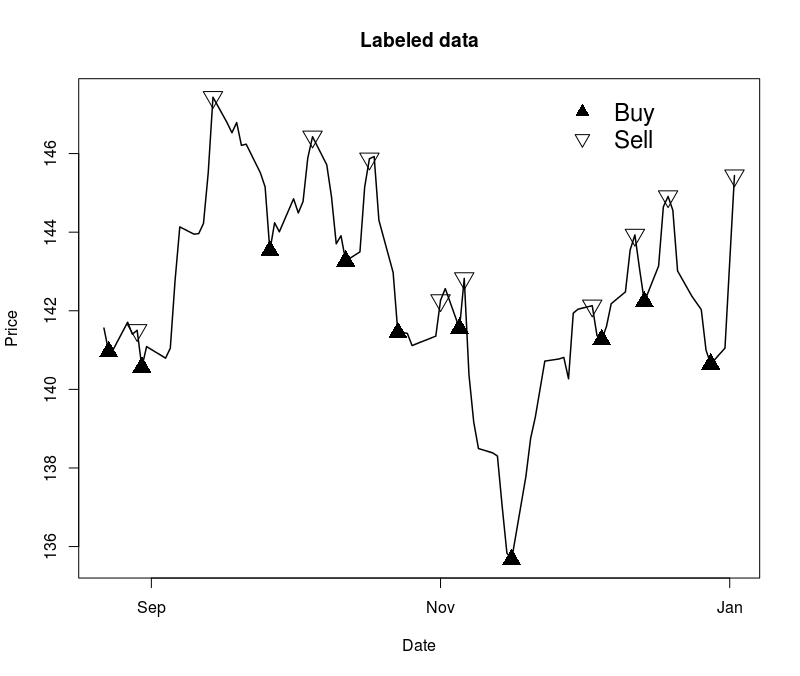
\includegraphics[width=1\linewidth]{images/labelling.jpeg}
\caption{\label{figure:Labelling} Labelled data set}
\end{figure}

\subsection{Incremental learning}
For both learning algorithms, AQ and CN2, we realized two type of experiments. The first of them is based on a \textit{learn-apply-discard} approach, in which, given a training set, we induce a set of rules and apply them to the closest test set. After that, we discard these set of rules (forget mechanism).

The other approach is based on an \textit{incremental learning} methodology, in which we learn a set of rules and instead of discarding them we order them according to their performance over the training set from which they were induced for the first time and their performance over the test sets in which they were used, keeping just a \textit{top k} of buy rules and a \textit{top k} of sell rules.

For measuring rule's performance over a training set we use the sum of their \textit{support} and their \textit{Laplace accuracy}.

On the other hand, for measuring rule's performance over a test set and in order to consider the non-stationary behaviour of stock markets, we reward (penalize) a pair of buy-sell rules, if their interaction involved a gain (loss).

The reward (penalization) given to each pair of buy-sell rules in a buy-sell transaction, is the percentage gain (loss) they caused, that is:

\begin{equation} \label{eqn:reward}
reward(B,S) = \dfrac{P_{sell} }{P_{buy}} -1 
\end{equation}

where $reward(B,S)$ is the reward (or loss) for a pair of buy-sell rules in a buy-sell transaction and $P_{sell}$, $P_{buy}$, are the sell and buy price respectively.

Finally for each rule that did not appear in the test set being evaluated, we penalize it with the average loss over that same test set, this acts as a way for discarding rules due to the pass of time.

Thus, the score for a rule, $R$, before the test set $M$, is given by:

\begin{equation} \label{eqn:rule-score}
score_{t}(R) = support + Laplace + \sum_{i} rewards_{i}
\end{equation}

where $support$ and $Laplace$ are, respectively, rule's support and its Laplace accuracy, both as measured in the training set from which the rule was induced for the first time. The sum in equation (\ref{eqn:rule-score}) includes all the test sets that appear after the first training set where the rule $R$ is induced and up to (excluding) the $M$-th test.

In this way, we are able to keep past and present knowledge and also identify sets of useful rules while discarding the ones that caused losses.

Figure \ref{figure:Incremental-learning} shows the process of incremental learning. For all the experiments the value of $K$ is set equal to $5$.
\begin{figure}[h]
\centering
\scalebox{0.5}{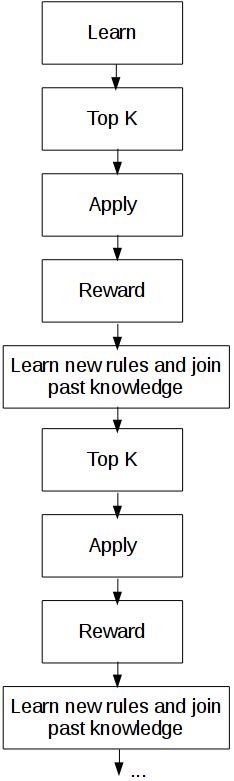
\includegraphics[width=1\linewidth]{images/incremental-learning.png}}
\caption{\label{figure:Incremental-learning} Incremental learning}
\end{figure}

\subsection{Sell limit orders}
\label{subsec:limit orders}
In addition to the sell rules induced by each algorithm, we add two more rules whose purpose is to capture investor's risk profile.

These new rules are related to sell limit orders and work by setting two limits corresponding to rising and falling markets.

The rules are triggered depending on the variation between the execution price and the achieved price of the most recent buy transaction as shown in equation (\ref{eqn:price-variation}).

\begin{equation} \label{eqn:price-variation}
variation = \dfrac{P_{exec}  (1 - c) }{P_{buy} (1 + c) } - 1
\end{equation}

where $c$ is the transaction cost percentage.

Thus, a sell signal is triggered when one of the following conditions is met:

\begin{align}
R_{sell} \wedge (variation > UL) \label{eqn:Sell-rule 1}\\
R_{sell} \wedge (variation < LL) \label{eqn:Sell-rule 2S}
\end{align}

where $R_{sell}$ is a sell rule induced by a learning algorithm and $UL$, $LL$ are the user defined upper and lower limits respectively.

Figure \ref{figure:Sell limits} shows the sell limits for a specific buy order.
\begin{figure}[h]
\centering
\scalebox{1}{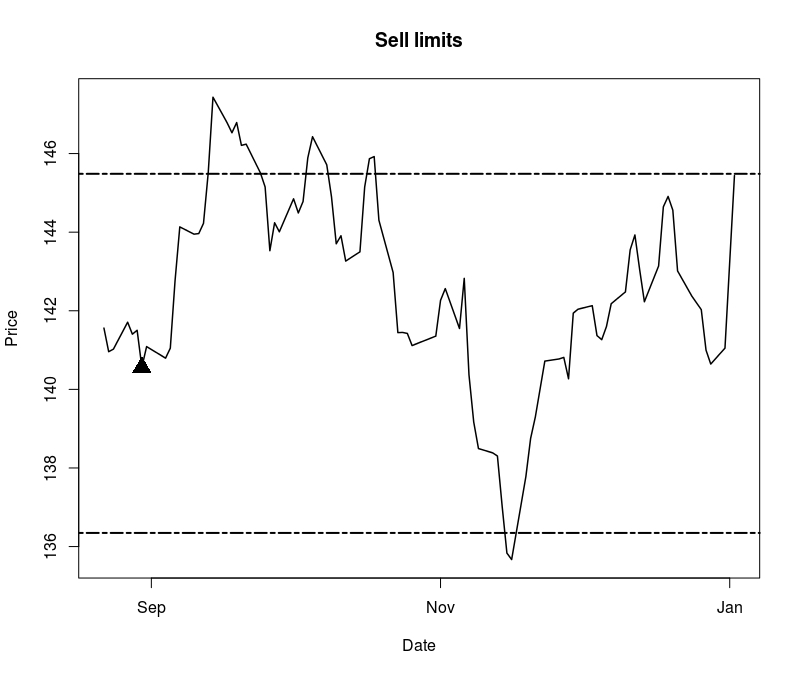
\includegraphics[width=1\linewidth]{images/sell_limits.jpeg}}
\caption{\label{figure:Sell limits} Sell limits}
\end{figure}

\subsection{Trading assumptions}
\label{subsec:trading-assumptions}
For every experiment the following trading assumptions are made:

\begin{itemize}
\item Given a buy or sell signal at time $t$, its execution is realized at time $t+1$ and the execution price is the mid price (average of low and high price) at $t+1$.

\item The transaction cost per operation is set equal to $0.25\%$. Thus for a buy transaction we end up paying:
$$ P_{buy} (1 + 0.0025)$$
per stock. Whereas for a sell transaction we receive:
$$ P_{sell} (1 - 0.0025)$$ 
per stock.

\item For a buy signal, we buy as many stocks as we can afford with our current capital. Likewise for a sell signal we sell all the stocks held at that time.

\item We can only sell something that we own, that is, we don't allow short sales.

\item The upper sell limit is equal to 0.035 or $3.5\%$ relative to the most recent buy price.

\item The lower sell limit is equal to -0.03 or $-3.0\%$ relative to the most recent buy price.

\end{itemize}


\section{Results}
\label{sec:results}
Using the methodology and trading assumptions explained in section \ref{sec:proposed methodology}, we realized four experiments for each learning algorithm. These experiments explore two types of discretization methods, unsupervised intervals (UI) and unsupervised quantiles (UQ).

Each discretization method uses both learning approaches, incremental learning (IL) and learn-apply-discard (LD).

For every test set the excess return over the buy-and-hold strategy and the total monetary gain for every \$100,000.00 invested, are calculated. Tables \ref{table:AQ results} and \ref{table:CN2 results} show the results.

As we can see, AQ algorithm is able, on average, to outperform buy-and-hold strategy when using incremental learning.

On the other hand, CN2 algorithm performs poorly in all the scenarios, the reason behind this, is because even when CN2 by default gives us an ordered set of rules, we're breaking that order when rewarding (penalizing) rules performance over the test sets.

Despite these results, is important to notice that two test sets comprise the $2008$ financial crisis, namely, the test sets for the periods $2008/05/12$ - $2008/09/17$ and $2008/09/18$ - $2009/01/27$.

As we can see from tables \ref{table:AQ results for 2008} and \ref{table:CN2 results for 2008}, specially for the period $2008/09/18$ - $2009/01/27$, we have very large excess returns but this fact is due merely to the bearish (trending down) nature of the market in that period, as signalled in \cite{Lohpetch2010}, the real challenge is beating the buy-and-hold strategy when markets are trending up.

Thus we recalculated the performance of each algorithm by excluding $2008$ financial crisis period,  the results are shown in tables \ref{table:AQ results without 2008} and \ref{table:CN2 results without 2008}.

As we can see, our excess returns are now negatives, nonetheless AQ algorithm with incremental learning is still the best approach among the others. 

Also worth noting that none of the approaches caused a negative average monetary gain.

\begin{center}
\begin{table*}[ht]
\centering
\begin{tabular}{ccccc}
\hline
\textbf{AQ} & \textbf{IL-UI} & \textbf{LD-UI} & \textbf{IL-UQ} & \textbf{LD-UQ} \\
\hline
Average excess return & $0.37\%$ & $-0.39\%$ & $0.20\%$ & $-1.02\%$ \\
\# Positive excess returns & $11$ & $14$ & $10$ & $13$  \\
\# Negative excess returns & $19$ & $16$ & $20$ & $17$ \\
Max excess return & $34.64\%$ & $22.17\%$ & $29.72\%$ & $20.3\%$ \\
Min excess return & $-11.23\%$ & $-12.94\%$ & $-3.86\%$ & $-11.47\%$ \\
Average monetary gain & $\$2,384.18$ & $\$1,620.11$ & $\$2,214.84$ & $\$ 994.96$ \\
\hline
\end{tabular}
\caption{\label{table:AQ results} Results for AQ algorithm}
\end{table*}
\end{center}

\begin{center}
\begin{table*}[t]
\centering
\begin{tabular}{ccccc}
\hline
\textbf{CN2} & \textbf{IL-UI} & \textbf{LD-UI} & \textbf{IL-UQ} & \textbf{LD-UQ} \\
\hline
Average excess return & $-1.22\%$ & $-1.07\%$ & $-0.54\%$ & $-1.41\%$ \\
\# Positive excess returns & $11$ & $10$ & $12$ & $8$  \\
\# Negative excess returns & $19$ & $20$ & $18$ & $22$ \\
Max excess return & $15.69\%$ & $12.32\%$ & $11.81\%$ & $6.05\%$ \\
Min excess return & $-12.87\%$ & $-9.43\%$ & $-6.48\%$ & $-8.33\%$ \\
Average monetary gain & $\$792.43$ & $\$946.07$ & $\$1,475.04$ & $\$ 604.99$ \\

\hline
\end{tabular}
\caption{\label{table:CN2 results} Results for CN2 algorithm}
\end{table*}
\end{center}

\begin{center}
\begin{table*}[t]
\centering
\begin{tabular}{ccccc}
\hline
\textbf{AQ for 2008} & \textbf{IL-UI} & \textbf{LD-UI} & \textbf{IL-UQ} & \textbf{LD-UQ} \\
\hline
$2008/05/12$ - $2008/09/17$ & $8.13\%$ & $2.33\%$ & $6.14\%$ & $3.57\%$ \\
$2008/09/18$ - $2009/01/27$ & $34.64\%$ & $22.17\%$ & $29.72\%$ & $20.37	\%$  \\
\hline
\end{tabular}
\caption{\label{table:AQ results for 2008} Results for AQ algorithm, 2008 financial crisis period}
\end{table*}
\end{center}

\begin{center}
\begin{table*}[t]
\centering
\begin{tabular}{ccccc}
\hline
\textbf{CN2 for 2008} & \textbf{IL-UI} & \textbf{LD-UI} & \textbf{IL-UQ} & \textbf{LD-UQ} \\
\hline
$2008/05/12$ - $2008/09/17$ & $0.27\%$ & $-0.38\%$ & $5.06\%$ & $-2.81\%$ \\
$2008/09/18$ - $2009/01/27$ & $15.69\%$ & $12.32\%$ & $11.81\%$ & $-0.62\%$  \\
\hline
\end{tabular}
\caption{\label{table:CN2 results for 2008} Results for CN2 algorithm, 2008 financial crisis period}
\end{table*}
\end{center}

\begin{center}
\begin{table*}[ht]
\centering
\begin{tabular}{ccccc}
\hline
\textbf{AQ without 2008} & \textbf{IL-UI} & \textbf{LD-UI} & \textbf{IL-UQ} & \textbf{LD-UQ} \\
\hline
Average excess return & $-1.13\%$ & $-1.29\%$ & $-1.06\%$ & $-1.94\%$ \\
\# Positive excess returns & $9$ & $12$ & $8$ & $11$  \\
\# Negative excess returns & $19$ & $16$ & $20$ & $17$ \\
Max excess return & $2.33\%$ & $6.84\%$ & $2.30\%$ & $1.85\%$ \\
Min excess return & $-11.23\%$ & $-12.94\%$ & $-3.86\%$ & $-11.47\%$ \\
Average monetary gain & $\$2,774.11$ & $\$2,608.11$ & $\$2,839.54$ & $\$1,958.46$ \\
\hline
\end{tabular}
\caption{\label{table:AQ results without 2008} Results for AQ algorithm without 2008 financial crisis}
\end{table*}
\end{center}

\begin{center}
\begin{table*}[ht]
\centering
\begin{tabular}{ccccc}
\hline
\textbf{CN2 without 2008} & \textbf{IL-UI} & \textbf{LD-UI} & \textbf{IL-UQ} & \textbf{LD-UQ} \\
\hline
Average excess return & $-1.88\%$ & $-1.57\%$ & $-1.18\%$ & $-1.38\%$ \\
\# Positive excess returns & $9$ & $9$ & $10$ & $8$  \\
\# Negative excess returns & $19$ & $19$ & $18$ & $20$ \\
Max excess return & $4.32\%$ & $9.52\%$ & $2.15\%$ & $6.05\%$ \\
Min excess return & $-12.87\%$ & $-9.43\%$ & $-6.48\%$ & $-8.33\%$ \\
Average monetary gain & $\$2,026.16$ & $\$2,334.63$ & $\$2,725.17$ & $\$2,517.75$ \\
\hline
\end{tabular}
\caption{\label{table:CN2 results without 2008} Results for CN2 algorithm without 2008 financial crisis}
\end{table*}
\end{center}


\section{Discussion and conclusions}
\label{sec:conclusions}
%Are rules financial coherent?
%Future work (other formulae for rewards)

\bibliography{references}
\bibliographystyle{elsarticle/elsarticle-harv.bst}


\end{document}